\documentclass[11pt]{article}

% ---------- Layout ----------
\usepackage[letterpaper,margin=1in]{geometry}
\usepackage{setspace}
\setstretch{1.05}

% ---------- Math & text ----------
\usepackage{amsmath,amssymb}
\usepackage{microtype}

% ---------- Figures & tables ----------
\usepackage{graphicx}
\usepackage{float}
\usepackage{booktabs}
\usepackage{caption}

% ---------- Links ----------
\usepackage[colorlinks=true,linkcolor=blue,citecolor=blue,urlcolor=blue]{hyperref}

% ---------- Bibliography (choose one) ----------
% If you use biblatex:
% \usepackage[backend=biber,style=authoryear]{biblatex}
% \addbibresource{references.bib}

% If you use natbib:
\usepackage[authoryear]{natbib}



% ---------- Title block ----------
\title{The Ideological Embeddedness of Macroeconomic Indicators: \\
Capacity Utilization Measurements in the Rise and Fall of American Keynesianism\thanks{This paper benefited from AI-assisted editing using Qwen3.6 Plus for syntax refinement, structural suggestions, and stylistic consistency checks. All analytical arguments, historical interpretations, and substantive content remain the author's sole responsibility.}}
\author{Diego Polanco\thanks{Doctoral Candidate in Economics, Department of Economics, University of Massachusetts Amherst.}\\
Department of Economics, University of Massachusetts Amherst\\
\texttt{dpolanconeco@umass.edu}}


\begin{document}
\maketitle

\begin{abstract}
This article traces how \textit{capacity utilization}---a statistic once central to Keynesian demand management---was redefined amid the Fordist crisis and the collapse of American Keynesianism. Focusing on the United States from the 1930s to the 1970s, I show how survey instruments, institutional venues (the Brookings Institution, McGraw--Hill, and the Federal Reserve), and political choices co-produced the operational routines through which economic slack became legible to policymakers. The core claim is that capacity utilization shifted from a Keynesian slack indicator for mobilizing idle resources to a neoliberal inflation sentinel used to discipline distributive conflict. This recoding was not a clean theoretical break but a strategic redeployment of existing methodological tools: the optimization--stability apparatus of the neoclassical synthesis, once used to justify discretionary management, was repurposed to enforce credibility-based rules when stagflation exposed the limits of demand management. Methodologically, I treat macroeconomic indices as contested socio-technical devices---not neutral mirrors of the economy but infrastructures that condition what policy problems are visible and actionable. Empirically, the paper reconstructs how survey-based capacity-utilization measures gained institutional authority while engineering-based alternatives were marginalized. The conclusion reflects on what recovering plural measurement practices might mean for democratic contestation in macroeconomic governance today.
\end{abstract}

\vspace{1cm}

\noindent\textbf{Keywords:} Capacity Utilization; American Keynesianism; Fordism; Macroeconomic Measurement; Ideology.

\noindent\textbf{JEL Codes:} E01; E32; B22; N12; P16.

\pagebreak

\section{Introduction}

Scholars of American Keynesianism have long debated its intellectual architecture and policy legacies, yet the statistical infrastructure that made Keynesian demand management operational remains underexamined. This article reassesses the fall of American Keynesianism by tracing the institutional history of capacity utilization measurement. I argue that the shift from postwar demand management to neoliberal credibility was not driven solely by theoretical innovation or political reaction, but by the ideological embeddedness of macroeconomic indicators. Between the 1930s and 1970s, capacity utilization was systematically recoded from a Keynesian slack indicator---used to identify idle resources and justify expansionary policy---into an inflation sentinel that disciplined distributive conflict and narrowed the space for egalitarian claims. This transformation did not occur through a clean paradigm rupture. Rather, it emerged from the strategic redeployment of existing technocratic tools: the same optimization frameworks and survey routines that had stabilized the postwar class compromise were repurposed to enforce market discipline when stagflation exposed the limits of discretionary governance.

Recent overviews have mapped the conceptual terrain of capacity utilization from two angles: evolutionary reconstructions of its theoretical genealogy \citep{trezzinipignalosa2024} and heterodox debates over the endogeneity of normal utilization rates \citep{nikiforos2016}. While these contributions clarify theoretical disputes, they leave the institutional and political economy dimensions underexplored. This paper intervenes by treating capacity utilization not as an abstract variable but as a socio-technical device whose stabilization and re-purposing reflect concrete struggles over state power. I trace how private and public institutions---the Brookings Institution, McGraw--Hill, and the Federal Reserve---made one version of utilization operational for demand management during the Fordist era, and how that same apparatus was re-coded during the 1970s crisis. By locating measurement practices within their historical context, I show how technical statistics conditioned the institutional arena in which distributive conflict unfolded.

The article proceeds in three stages. First, it reconstructs pre-Keynesian measurement endeavors at the Brookings Institution, which established the engineering-versus-economic capacity distinction that would later inform policy dashboards. Second, it examines the postwar institutionalization of survey-based utilization measures, showing how McGraw--Hill's business intelligence routines gained Federal Reserve authority and crowded out physically anchored alternatives. Third, it analyzes the 1970s stagflation crisis as a critical juncture in which mainstream economists and policymakers reinterpreted high operating rates as inflationary warnings, thereby completing the shift from demand management to credibility-based discipline. The conclusion reflects on how recovering marginalized measurement practices can inform contemporary debates over macroeconomic governance.

This paper treats capacity utilization not as a neutral technical variable but as a politically contested measurement infrastructure. I situate the analysis within the political economy of macroeconomic statistics, drawing on scholarship that examines how quantitative indicators stabilize particular governance logics while marginalizing alternatives \citep{porter1995,block2008,krippner2011}. Rather than attempting to synthesize socio-technical, institutional, and intellectual history into a single framework, I subordinate these strands to a core question: how did survey-based utilization routines become authoritative, and how were they strategically repurposed during the 1970s crisis? Regulation theory and science-and-technology studies concepts appear here as contextual background rather than explanatory architecture. The Fordist/post-Fordist transition and the socio-technical character of measurement practices help situate the historical terrain, but the argument centers on institutional consolidation and ideological redeployment.

Methodologically, the paper combines conceptual history with institutional analysis. I trace how definitions of capacity were operationalized, benchmarked, and revised across Brookings reports, corporate surveys, and Federal Reserve releases. Following historical practice, I treat these documents as primary sources that require interrogation: who produced them, for what audience, and with what political or commercial purpose? This approach avoids treating measurement as a passive reflection of economic reality and instead reconstructs the compromises that granted one version institutional authority. The analysis also engages recent work in the history of economic thought and economic governance, situating American Keynesianism not as a coherent doctrine but as an evolving set of administrative practices conditioned by measurement constraints \citep{barber1987,backhouse2015}.

The remainder of the article unfolds chronologically to track this institutional trajectory. Section 2 examines pre-Keynesian measurement efforts at the Brookings Institution, which first rendered productive capacity legible to policymakers. Section 3 reconstructs the postwar consolidation of the pedagogy--policy corridor and the institutionalization of slack measurement. Section 4 analyzes how McGraw-Hill's business intelligence routines gained Federal Reserve authority and displaced engineering-based alternatives. Section 5 examines the 1970s stagflation crisis as a critical juncture in which mainstream economists and policymakers reinterpreted high operating rates as inflationary warnings, completing the shift from demand management to credibility-based discipline. The conclusion reflects on how this institutional history reframes contemporary debates over macroeconomic indicators and democratic governance.

\section{Pre-Keynesian Endeavors on Capacity Utilization Measurements}

The growing influence of Keynesian economic thought heightened concern with the business cycle and, correspondingly, with capacity utilization. Its early measurement in the United States did not originate in government statistics \footnote{Early industrial output statistics preceded Brookings and the later institutionalization of capacity utilization measurement: the Federal Reserve began publishing monthly production tables and introduced early industrial production indexes in 1919, but these series did not yet incorporate a notion of productive capacity. See \citep{bogfrs2017}.} or Keynesian policy shops but in a pragmatic, policy-oriented research program at the Brookings Institution, a private nonprofit founded by Robert S. Brookings. In the aftermath of the Great Depression, Brookings pioneered modern empirical practices in measurement, cross-sectoral analysis, and macro-policy reporting, including sectoral estimates of capacity utilization. The program culminated in a four-volume study published in the mid-1930s:
\begin{enumerate}
\renewcommand{\labelenumi}{\roman{enumi})}
\item \emph{America's Capacity to Produce} (1934),
\item \emph{America's Capacity to Consume} (1934),
\item \emph{The Formation of Capital} (1935), and
\item \emph{Income and Economic Progress} (1935).
\end{enumerate}

The first volume, \emph{America's Capacity to Produce}, was the earliest large-scale empirical attempt to measure capacity utilization in the United States. Working in a pre-Keynesian, American-institutionalist framework and organizing the analysis by economic sectors, \citet{nourseetal1934} distinguished three related notions of capacity utilization stated in operational terms:

\begin{enumerate}
\renewcommand{\labelenumi}{\roman{enumi})}
\item theoretical capacity, the engineering upper bound if plant runs continuously at rated speeds under ideal conditions (abstracting from maintenance and equipment turnover);
\item practical capacity, the maximum sustainable output under prevailing production conditions, given organizational norms, normal shift schedules, and effective working hours, excluding unavoidable interruptions and idle plants; and
\item capacity utilization, defined as the share of practical capacity actually used, with theoretical capacity serving as a benchmark.
\end{enumerate}
Macro-aggregation was reported as a weighted average of sectoral indices, adjusted by a discretionary factor to reflect intersectoral ``coordination failures.''

% ---------- Example figure insertion ----------
\begin{figure}[H]
   \centering
   \caption{Automobile Capacity and Production, 1902-1930}   
   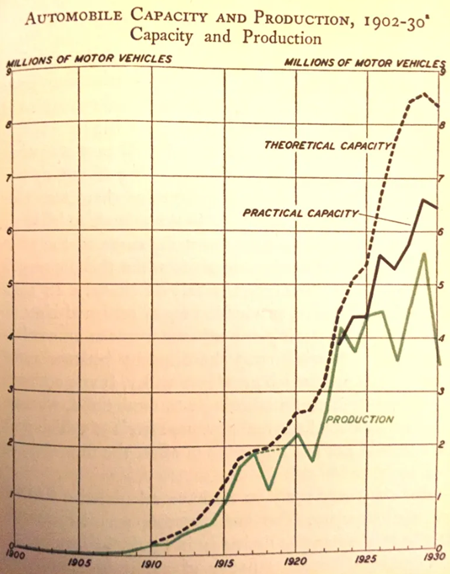
\includegraphics[width=0.5\linewidth]{figure1.png}
    \caption*{\small Source: \citet[p.229]{nourseetal1934} \textit{"America's Capacity to Produce". The Brookings Institution.}.}
   \label{fig:automobile_capacity}
\end{figure}

Methodologically, the project combined plant-level reports, industry surveys, and administrative series. Missing observations were addressed through documented statistical imputations to harmonize reported capacity and hours, with weights proportional to an establishment's rated capacity. Sectoral coverage extended beyond heavy industry to consumer durables and selected services, which helped explain heterogeneity in depth and data quality across sectors. The macro index was therefore an explicitly constructed statistic rather than a passive average: a transparency the authors highlighted as a virtue even while acknowledging discretion in benchmarks and weights.

Brookings reports demonstrated that the Depression reflected demand-side contractions, especially weak consumption, rather than physical production limits. These findings foreshadowed Keynes's \emph{General Theory} while eschewing its redistributive policy program. The Institution did not call for redistribution as a plausible policy pathway; instead, it recommended efficiency improvements and pricing reforms aimed at passing productivity gains to consumers via market mechanisms. Early assessments converged on this reading while drawing different boundaries on method and implication. \citet{davis1935} welcomed the first systematic sectoral study and its macro extrapolation but questioned arbitrary empirical choices and noted uneven depth across industries. \citet{ugge1936} praised the pragmatic approach, careful statistical treatment (including novel imputations), and wide industrial coverage, stressing the policy value of estimating idle resources. He also underlined the usefulness of standardized cost accounting and survey regularity for future business-cycle analysis. \citet{commons1937} situated the Brookings work within American institutionalism as incompatible with neoclassical full-employment theorizing. He praised its documentation of resource idleness as an empirical break with equilibrium orthodoxy. Nevertheless, at the same time, he criticized the program's reliance on price reductions over redistributive or macro-stabilization measures and the absence of an explicit demand-management mechanism to mobilize spare capacity.

As Commons implied, the United States of the 1930s offered fertile ground for a new doctrine of macroeconomic policy. Brookings' economists documented that the 1929 Wall Street crash left the economy with widespread underutilization, including a sharp 1930 production downswing alongside continued growth of productive capacities across sectors (including automobiles, as shown in Figure~\ref{fig:automobile_capacity}), inaugurating the decade of the Great Depression. That empirical baseline matters for what follows: capacity became legible to policy not because theory demanded it but because measurement infrastructures made economic slack visible, and available to debate for businessmen, economic elites, and politicians, setting the stage for the rise of a new economic paradigm: ``American Keynesianism'' alongside its institutionalization through different pathways. Here, I shall emphasize two entangled ones: the standardization of industrial surveys aimed to provide aggregate measurements of capacity utilization by the Federal Reserve during the post-war period, and the consolidation of Keynesian economic thinking in the United States through its dominance in the cultural landscape of research, teaching, and learning, fueled by an increasingly developed and robust higher education system.

\section{The Rise of Keynesianism with American Characteristics}

Alvin Hansen stepped in to fill this gap in American economic reasoning. By the time of the Great Depression, Hansen had already established himself as a leading business-cycle economist, publishing his dissertation, \emph{Cycles of Prosperity and Depression in the United States, Great Britain, and Germany} (1921) \citep{hansen1921}. He framed business cycles as endogenous to capitalist economies, assigning a central role to expectations, investment, and technological change. Depressions were not merely external shocks but the result of endogenous dynamics, including mismatches between the production and consumption of capital and consumer goods and the over-investment and lagged self-adjustments they triggered. Observing that the United States' dynamism, once driven by technological progress and territorial expansion, was dying down, he anticipated his later thesis on secular stagnation \citep{hansen1938}. As \citet{barber1987} emphasizes, Hansen's interwar work treated cyclical movements as endogenous adjustments within a capital accumulation process rather than as exogenous weather-like disturbances, a reading that helps explain his receptivity to policy design once a coherent stabilization framework became available after Keynes' \emph{General Theory} was published and widely debated across the world.

In his 1936 essay, ``Mr. Keynes on Underemployment Equilibrium,'' Hansen engaged Keynes's \emph{General Theory} with cautious skepticism while acknowledging the novelty of equilibrium with labor underemployment \citep{hansen1936}; Keynes, [1936] 2018. Between 1936 and 1938, he selectively adopted Keynesian tools to confront what he took to be the central empirical fact of the era: the persistence of idle resources, visible as mass unemployment and unused capacity \citep{barber1987}. Hicks's IS--LM formalization consolidated his conversion, providing a teachable toolkit that Hansen used to mobilize ideas in the classroom and in print, culminating in his formulation of secular stagnation as a diagnosis of the 1930s downturn \citep{hicks1937}. This is also where the measurement link begins to surface. The problem Hansen wanted to solve was not an abstract paradox but a practical one: how to diagnose and manage persistent slack. That required statistics that could register unused capacity and guide countercyclical action. Brookings' sectoral inquiries into capacity and the maturing Federal Reserve index of industrial production furnished early proxies, while business surveys began to report plant load ratios in a way legible to policymakers \citep{barber1987}.

This intellectual shift coincided with a move into policy and institution-building. In 1937, Hansen became the first Lucius N.\ Littauer Professor of Political Economy at Harvard's Graduate School of Public Administration. He combined Keynesian analysis with the data-minded habits of his early work and pursued an institution-building agenda \citep{musgrave1976}. That orientation shaped his pedagogy and federal advising, pushing Keynesian stabilization into mainstream policy. The pathway from Cambridge to Washington is clear: his 1939 testimony before the Temporary National Economic Committee (TNEC) legitimated deficit spending and set up his \emph{Fiscal Policy and Business Cycles} (1941), which (i) systematized countercyclical budgeting, (ii) linked bond finance and interest-rate pegs to real-side stabilization, and (iii) argued for automatic stabilizers and public investment as designed institutions rather than ad hoc fixes (TNEC 1939; \citealp{hansen1941}). Even though Hansen did not work directly on capacity utilization measurement, he became central to the statecraft that governed it. Musgrave's \citeyearpar{musgrave1976} portrait is telling: a scholar who coupled analytic tools to institutional imagination, translating classroom models into budget rules and administrative routines that required reliable indicators of slack.

Wartime and reconstruction widened this corridor. Advising Marriner Eccles at the Federal Reserve, Hansen supported rate pegs and bond finance \citep{bogfrs1945}. Through the National Resources Planning Board (NRPB) and the Council on Foreign Relations' War and Peace Studies, he helped craft full-employment planning and an external monetary architecture compatible with high domestic employment \citep{hansen1942,nerozzi2009}. In parallel, wartime planning normalized the practice of monitoring bottlenecks and capacity limits across industries, habituating agencies to think in terms of potential output and utilization rather than just prices and quantities \citep{bogfrs1945}. Domestically, this arc culminated in the Employment Act of 1946 and the creation of the Council of Economic Advisers (CEA), which made that commitment a continuing federal responsibility \citep{bailey1950}. In this way, American Keynesianism crystallized as a macroeconomic policy regime oriented toward demand management and, implicitly, the governance of capacity utilization. Samuelson later recalled Hansen as the leader of the ``Keynesian revolt'' that made Cambridge, Massachusetts, a hub of American Keynesianism \citep{samuelson1988}. In short, a feedback loop formed: pedagogy produced officials fluent in stabilization logics; those officials demanded operational statistics; those statistics, once institutionalized, reinforced the very style of macroeconomic governance that had prompted their creation.

Hansen's most prominent student, Paul Samuelson, developed a discrete-time model that synthesized Keynes's multiplier with Clark's accelerator, in which investment shocks, amplified by the multiplier, feed back through the accelerator to generate cyclical fluctuations \citep{samuelson1939,clark1917}; Keynes [1936] 2018. Guided by E.\ B.\ Wilson's methodological tutelage, Samuelson moved to {MIT} and completed the dissertation that became \emph{Foundations of Economic Analysis} (1947) \citep{samuelson1947}. \emph{Foundations} supplied the optimization--stability toolkit (including the correspondence principle) and quickly became a touchstone for graduate training \citep{backhouse2014,backhouse2015}. By contrast, his \emph{Economics: An Introductory Analysis} (1948) carried the undergraduate classroom, standardizing national-income accounting, the 45-degree Keynesian cross, and the Hicks--Hansen IS--LM reading \citep{samuelson1948,dimand2010,pearcehoover1995}. Together, \emph{Foundations} and \emph{Economics} provided the architecture and the pedagogical vehicle of what became the neoclassical--Keynesian synthesis, with Samuelson as its principal architect and diffuser \citep{davidson2006}. For measurement, this mattered: the 45-degree cross and IS--LM did not just inhabit lecture halls; they shaped what agencies asked the data to reveal about gaps between actual and potential output, and therefore how ``capacity'' would be operationalized in practice.

Read within U.S.\ higher education, \emph{Economics} had a broad cultural reach but was no neutral mirror of the discipline \citep{pearcehoover1995,colanderlandreth1996,colander2003}. Treating the textbook as an active agent clarifies how the ``neoclassical synthesis'' label was normalized for mass pedagogy \citep{devroey2004,backhouseboianovsky2016}. The same lens opens an internationalization angle: translations and adoptions, including early Japanese editions in the immediate postwar period, exported ``American economic reasoning'' directly into classrooms and into non U.S.\ academic cultures \citep{fourcade2009,giraud2018}. Concrete examples clarify the point. Early Japanese adoptions adapted the Keynesian toolkit to a reconstruction economy with explicit planning targets, folding utilization into industrial rationalization debates; in Western Europe, the same pedagogy interacted with indicative planning and social partnership institutions, where ministries and research institutes tracked capacity constraints as part of growth programs \citep{fourcade2009}. These variants underscore that the ``American'' synthesis traveled, but it did not land on neutral ground. Work on textbook-market dynamics also tempers the ``template'' myth: standardization emerged from mutual stabilization across competing texts, iterative revisions, and publisher incentives, not one-way imitation (\citealp{colander2003,giraud2018}). These textbook and publishing dynamics foreshadowed the postwar infrastructure for measurement---from Brookings' capacity studies to the McGraw--Hill utilization series---which the next section examines.

The final piece is institutional. By the late 1940s and 1950s, business press surveys (notably McGraw--Hill) were circulating plant capacity questions at scale, while the Federal Reserve refined the industrial production index as a backbone for cycle dating. Together they formed a usable dashboard for officials trained in the Hansen--Samuelson idiom: utilization rates to gauge slack, production indices to track momentum, and budget rules to respond. That ensemble made capacity utilization a governable object rather than a background condition, closing the loop opened by Hansen's interwar analysis.


\subsection{The Technocratic Corridor: Slack Measurement and the Institutionalization of American Keynesianism}
\label{subsec:technocratic_corridor}

The consolidation of American Keynesianism rested not only on theoretical innovation but on the construction of a pedagogy--policy corridor that translated classroom models into administrative routines. When Alvin Hansen moved to Harvard's Graduate School of Public Administration in 1937 and Paul Samuelson arrived at MIT in 1940, they created institutional nodes where stabilization logic was codified, taught, and disseminated to federal agencies \citep{barber1987,backhouse2015}. 

\citet{samuelson1948} \emph{Economics} did more than teach Keynesian cross diagrams; it trained a generation of officials who entered the Council of Economic Advisers, Federal Reserve, and Treasury expecting macroeconomic management to be a technical problem of optimizing within constraints \citep{pearcehoover1995}. That expectation created demand for operational indicators of slack---reliable measures of capacity utilization that could guide counter-cyclical policy \citep{musgrave1976}. Once embedded in the Federal Reserve's G.17 release and CEA reports, those survey-based measures reinforced the very style of technocratic governance that had prompted their creation. 

But this feedback loop carried an implicit political valence. The neoclassical synthesis Samuelson championed \citep{samuelson1947,samuelson1948} framed distributional conflict as an externality to be managed rather than a constitutive feature of capitalist politics. As Block notes, that technocratic ethos narrowed the space for egalitarian policy experimentation even as it stabilized capital accumulation under a fragile class compromise \citep{block2008,jessop2002}. The postwar institutionalization of capacity utilization measurement thus reflected not only epistemic consensus but also the strategic selectivity of a state apparatus oriented toward managing, not transforming, the terms of accumulation.

This corridor operated through concrete administrative practices. Officials trained in Hansen--Samuelson models required statistics that could register unused capacity and guide intervention. Brookings' sectoral inquiries, the maturing Federal Reserve index of industrial production, and emerging business surveys furnished early proxies \citep{barber1987}. By the late 1940s, the practice of monitoring bottlenecks and capacity limits across industries had become routine, habituating agencies to think in terms of potential output and utilization rather than just prices and quantities \citep{bogfrs1945}. The Employment Act of 1946 and the creation of the Council of Economic Advisers made full-employment commitment a continuing federal responsibility \citep{bailey1950}, which in turn required reliable indicators of slack. 

In this way, American Keynesianism crystallized as a macroeconomic policy regime oriented toward demand management and, implicitly, the governance of capacity utilization. The feedback loop was complete: pedagogy produced officials fluent in stabilization logics; those officials demanded operational statistics; those statistics, once institutionalized, reinforced the very style of macroeconomic governance that had prompted their creation. This institutional embedding of slack measurement would prove decisive when stagflation exposed the limits of discretionary policy: the same apparatus did not disappear but was repurposed, as the next section shows.

\subsection{Survey Infrastructure and the Institutionalization of Capacity Utilization}
\label{subsec:survey_infrastructure}

The postwar consolidation of capacity utilization measurement did not emerge from theoretical consensus but from the institutional consolidation of survey routines. When McGraw--Hill launched its annual plant-and-equipment survey in 1948, it did not produce a neutral technical artifact. The questionnaire asked managers to report actual operating rates alongside a ``preferred'' benchmark near 90 percent, a framing that naturalized corporate perspectives as statistical fact \citep{butler1958,phillips1963}. Produced for a business audience and disseminated through financial information networks, the series quickly became the most systematic private indicator of economic slack. Its authority rested not on engineering precision but on institutional reach: the survey's horizontal expansion into sectoral intelligence, testing, and broadcasting positioned McGraw--Hill as a central node in postwar business infrastructure \citep{munroe2007,baransweezy1988}.

Federal adoption followed path dependence, not methodological superiority. By the late 1950s, the Federal Reserve's Division of Research and Statistics embedded McGraw--Hill's operating-rate benchmarks into the Industrial Production program and disseminated results via the G.17 release \citep{bogfrs2017}. The choice reflected administrative convenience and coverage, not conceptual clarity. Survey responses remained managerial assessments rather than cost-minimizing constructs or engineering specifications, embedding subjective expectations into an index intended to guide stabilization policy. Contemporary critiques by \citet{butler1958} and \citet{phillips1963} noted this vulnerability, while \citet{kleindavid1958} and the Wharton Trend-Through-Peaks (TTP) procedure offered technically rigorous alternatives grounded in interindustry linkages and observed output peaks \citep{kleinsummers1967}. Yet the Fed retained the survey benchmark, institutionalizing a politically legible measure over analytically precise ones.

The marginalization of physically anchored alternatives illustrates the strategic selectivity of postwar statistical infrastructure. Indices like \citet{foss1963}'s Electric Motors Utilization (EMU) and \citet{taubmangottschalk1971}'s Average Workweek of Capital (AWW) tracked capital intensity, multiple shifts, and operational realities on the shop floor. Both consistently registered higher utilization rates and earlier cyclical turning points than the Federal Reserve series, aligning more closely with Keynesian concerns about cost dynamics and stabilization. Their failure to gain institutional adoption was not empirical but political: path dependence within the Fed's Industrial Production program, combined with the post-1970s turn toward NAIRU and output-gap frameworks, favored smooth series compatible with inflation targeting. Survey benchmarks had already been woven into administrative routines, making switching costs prohibitive even as conceptual tensions persisted.

Later assessments of \emph{America's Capacity to Produce} converge on a familiar verdict: despite its seminal status, the study lacked firm methodological foundations. \citet{burns1954} noted that \citet{nourseetal1934} conflated an economic definition of capacity with an engineering one, rendering policy prescriptions to mobilize idle capacity questionable. \citet{kleindavid1958} echoed this concern, identifying Brookings' estimates as explicitly engineering measures of capacity utilization. They further observed that statistical compilations were not standardized and that any aggregation from sectors to the macro level required an input--output consistent framework if one hoped to capture the intersectoral ``coordination failures'' that Nourse emphasized without resorting to arbitrary adjustments.

This gap spurred private-sector efforts in the late 1940s that surveyed firms directly. \emph{Fortune} magazine produced occasional capacity estimates based on survival-curve reconstructions derived from tax-based investment data. Contemporary commentators highlighted the lack of transparency and standardization in its methods and the large discrepancies relative to other survey-based measures \citep{butler1958,phillips1963}. While \emph{Fortune} helped insert the concept of capacity utilization into business discourse and tied it more closely to an economic rather than purely engineering notion, the resulting series were too fragile for rigorous research.

In the late 1940s, McGraw--Hill pursued a dual trajectory that proved decisive: the diffusion of Keynesian pedagogy and the construction of systematic business surveys. As Samuelson (1999) recalls, the firm was already a major academic publisher positioned to bring \emph{Economics} (1948) to a mass audience, thereby codifying postwar American Keynesianism. At the same time, McGraw--Hill leveraged its expanding business information services to collect empirical data, positioning itself at the intersection of pedagogy and measurement. Its corporate strategy was marked by a wave of acquisitions that consolidated a platform for publishing, information services, and broadcasting. These moves exemplify what \citet{baransweezy1988} describe as the informational and financial infrastructures characteristic of monopoly capitalism, consolidated with McGraw--Hill Co.\ acquisition of Standard \& Poor's financial services in 1966.

\begin{table}[h!]
\centering
\caption{McGraw--Hill Acquisitions, 1950--1972}
\label{tab:mcgrawhill_acquisitions}
\begin{tabular}{rp{4cm}p{5cm}}
\toprule
Year & Company acquired & Sector \\
\midrule
1950 & Gregg Company & Vocational textbooks (education publishing) \\
1953 & Platts Company & Petroleum industry information \\
1954 & Blakiston (from Doubleday) & Medical textbooks \\
1961 & F.\ W.\ Dodge Corporation & Construction industry information \\
1965 & California Test Bureau & Educational testing systems \\
1966 & Standard \& Poor's & Financial services \\
1966 & Shepard's Citations & Legal publishing \\
1968 & National Radio Institute & Correspondence school and broadcasting training \\
1970 & The Ryerson Press & Educational and trade publishing \\
1972 & Television Stations of Time Life Broadcasting & Broadcasting assets \\
\bottomrule
\end{tabular}
\captionsetup{font=small}
\caption*{Source: Author's elaboration based on \citet{munroe2007}.}
\end{table}

The acquisition pattern reveals a deliberate expansion across publishing, testing, financial intelligence, and broadcasting. Taken together, these moves embedded McGraw--Hill within multiple knowledge infrastructures, transforming the firm from a textbook publisher into a systematic producer of business intelligence. That infrastructure mattered for measurement: when the Federal Reserve later sought a reliable benchmark for industrial slack, McGraw--Hill's survey offered broad coverage, regular publication, and a format already familiar to corporate planners. The Fed's adoption thus reflected administrative convenience and institutional reach as much as methodological rigor, setting the stage for the survey's political elevation and the marginalization of technically precise alternatives.

The surveys' influence nevertheless drew methodological critique. \citet{butler1958} documented the business-cycle sensitivity of reported operating rates and warned that responses reflected managerial expectations rather than standardized definitions. \citet{phillips1963} criticized the reliance on subjective and heterogeneous capacity concepts and highlighted problems of aggregation and reproducibility. He also underscored weaknesses in the Federal Reserve's subsequent regression approach, which blended industrial production, McGraw--Hill series, and capital-stock estimates, contrasting it with the Wharton ``Trend-Through-Peaks'' (TTP) interpolation rule. These debates illustrated a broader search, amid the ascent of econometrics, for more formal and analytically grounded methods (Lou{\c{c}}{~a}, 2007).

The Wharton Trend-Through-Peaks (TTP) procedure offered one influential response. It constructed a path of productive capacities by interpolating between observed output peaks, defining utilization as the ratio of actual output to the interpolated path of productive capacities anchored in output peaks identified through TTP analysis. By construction, it delivered a conservative benchmark with no long-run trend in utilization, thereby limiting the temptation to read structural change into cyclical noise \citep{kleinsummers1967}. Building on this, \citet{kleindavid1958} also proposed an explicitly economic definition: capacity is the output that minimizes average cost, so that utilization is actual output divided by this cost-minimizing level. To scale from sectors to the aggregate without logical inconsistencies, they suggested an input--output consistent calibration in which the Leontief system is expanded up to the point at which sectoral capacity constraints bind, yielding a macro utilization index that respects interindustry linkages.

By the late 1950s, the Federal Reserve had incorporated McGraw--Hill's operating rate benchmarks into its statistical apparatus, extending the official capacity utilization index back to 1948. This move reflected the relative availability and coverage of the McGraw--Hill data compared with fragile alternatives and marked the institutional consolidation of survey benchmarks within the Keynesian State \citep{jessop2002}. The Division of Research and Statistics embedded the series in the Industrial Production program and disseminated results via the G.17 release \citep{bogfrs2017}. Periodic assessments acknowledged the policy relevance of survey-based indicators while also noting their conceptual limitations and the case for model-based complements \citep{usgao1996}.

The conceptual tensions that motivated these reforms did not vanish. Because ``capacity'' in surveys continued to reflect managerial assessments rather than engineering specifications or cost-minimizing constructs, comparability over time remained problematic. Smoothing, benchmarking, and revisions could add mean-reverting tendencies, while shifts in what managers regarded as ``normal'' operations risked embedding sentiment into an index intended to guide stabilization policy. In short, the official measures rested on theoretical priors as much as on directly observed production capabilities.

Alternatives, therefore, sought to anchor utilization in observable indicators of capital services. \citet{foss1963} developed the Electric Motors Utilization (EMU) index, comparing actual electricity consumption with theoretical consumption implied by installed motor horsepower. EMU captured intensity of use, including multiple shifts that became characteristic of mid-century Fordism, and it typically registered higher utilization than the Federal Reserve index. \citet{taubmangottschalk1971} introduced the Average Workweek of Capital (AWW), defining capital services as a function of shifts, hours per shift, and the share of the capital stock active in each shift. Quarterly estimates for 1952--1968 revealed turning points and volatility patterns distinct from the FRB measure, often yielding earlier signals of cyclical upswings and a closer match to operational realities on the shop floor. Both approaches emphasized how intensively capital was worked, rather than how much capacity managers reported usage of productive capacities, thereby aligning more closely with Keynesian concerns about cost dynamics and stabilization.

Despite their conceptual clarity and empirical appeal, EMU and AWW failed to secure institutional adoption. Path dependence within the Federal Reserve, where survey benchmarks had already been integrated into the Industrial Production program, implied high switching costs. The post-1970s policy turn toward NAIRU, output-gap frameworks, and production function estimates of potential output favored smooth series compatible with inflation targeting regimes, leaving physical indicators at the margins of economic debate. Even so, the research lineage persisted: \citet{foss1981} and \citet{foss1985} and subsequent work on capital services extended the physical indicator tradition, while heterodox analyses integrated utilization into broader narratives of long waves and profitability. From a Marxist perspective, \citet{shaikh1992} combined his previously developed critical assessment of neoclassical theory \citep{shaikh1974} with empirical series to expose the fragility of survey-grounded and neoclassical capacity concepts. Late Keynesian and early Post-Keynesian attempts to rehabilitate utilization measurement in the post Fordist era include \citet{orr1989}, \citet{beaulieumattey1998}, and more recently \citet{nikiforos2016}, sustaining an alternative tradition rooted in physical indicators in contrast to the institutionalized official survey-based approach.

This institutional consolidation set the stage for the 1970s recalibration. Once embedded in the Federal Reserve's statistical apparatus and CEA reporting practices, survey-based capacity utilization functioned as a thermostat for demand management. When stagflation exposed the limits of discretionary policy, the same apparatus did not disappear; it was repurposed. The shift from slack indicator to inflation sentinel did not require new measurement tools, only a new political economy of interpretation. The next section traces how mainstream economists and policymakers redeployed this existing infrastructure to discipline distributive conflict and narrow the space for egalitarian claims.


\section{The Crisis of Atlantic Fordism and the Fall of American Keynesianism}

Scholars have interpreted the postwar period as a distinct stage of historical capitalism, characterized by mass production coupled with mass consumption through an institutional wage-productivity nexus that stabilized growth across sectors \citep{aglietta2000}. Building on this perspective, \citet{vidal2015} situates ``Atlantic Fordism'' as a multi-scalar hegemonic bloc that bound together nationally specific class compromises across the North Atlantic geographical sphere into a coherent, U.S.-centered anchored order at the core of the capitalist world system.

Within this framework, \citet{jessop2002} emphasizes the Keynesian State as the institutional form of the State in core geographies of the world market, embedding demand-management practices in state projects that sustained full employment, intervened the economy with strong regulation, and enhanced social reproduction through welfare policies. The financing of social reproduction rested on a complementary balance among employers, households, and the public sector: wages covered a substantial share, while female unpaid household labor and the Keynesian State reinforced this arrangement through a social wage in form of government expenditures as social aid and public services \citep{moos2021}. The stability of this configuration also relied on the Bretton Woods system, which \citet{vernengo2021} interprets as a financial architecture that consolidated U.S. hegemony placing a key role in the Marshall Plan  for European reconstruction and financial aid to the development of Asian countries---such as Japan and Taiwan---as a geopolitical strategy to contain communist advance. Taken together, these accounts underscore how Fordism cannot be reduced to a purely national settlement but must be understood as a historically specific accumulation regime supported by multilevel institutional and financial arrangement with Keynesianism as an economic rationality embedded in different modalities and pathways, with historically contingent interpretations, critiques, and adaptations of Keynes original formulations in \emph{General Theory}\footnote{Keynes' \emph{General Theory} became a cornerstone for critical interpretations around the world. As has been argued before, Alvin Hansen was critical of Keynes in the first instance but embraced Keynesianism to become its main figure in the United States. The publication of \emph{A Guide to Keynes} in 1953 became the consolidation of his personal trajectory in becoming the pivotal figure of ``American Keynesianism.'' Parallelly, Ra{\'u}l Prebisch, the Argentinian director of the Economic Commission for Latin America and the Caribbean (ECLAC), would become known as the ``Latin American Keynes,'' while being critical of some aspects of the \emph{General Theory}. According to \citet{caldenteyvernengo2016}, the qualitative difference of Prebisch relative to Keynes were on dynamics and the cycle from an angle of the capitalist periphery from a global perspective, issues that were peripheral to Keynes' central message. In contrast to Hansen, Prebisch departed from his publication of \emph{Introducci{\'o}n a Keynes} in 1947 to becoming the pivotal figure of a Keynesianism in Latin America and beyond through the global south \citep{prebisch1947}. These parallel intellectual developments showcase that ``Keynesianism'' was an intellectual phenomenon of an epoch, with different interpretations and adaptations through different geographies, with their own and unique characteristics.}

Fordism hit its limits as the productivity--wage nexus increasingly delinked. With a shrinking reserve army and intensified wage militancy, profits were squeezed \citep{weisskopf1979}. U.S.-invited postwar development in Germany and Japan enabled a geopolitically enabled but non-expected catching-up that threatened U.S.\ market leadership \citep{lipietz1987,vidal2019geriatric}. While profits squeezed, profitability was sustained with rising capacity utilization \citep{weisskopf1979,shaikh2016}. Once stagflation emerged, it exposed the fragility of discretionary demand management and the incapacities of ``Keynesianism of American characteristics'' to manage demand and provide a fix to the crisis \citep{shaikhetal1999}.

\citet{moos2021} makes clear that a growing gap between the cost of reproducing labor power and employer compensation was temporarily stabilized by the Keynesian State, which socialized part of the burden through transfers, services, and regulation, a policy-packaged mostly known as ``the Great Society.'' This temporal fix sustained Fordism's class compromise into the early 1970s but could not be reproduced indefinitely within that institutional form, leaving the problem to resurface in the broader profitability and stagflation crisis. In this scenario, ideological struggles over what `capacity utilization' measured became openly contested. In this sense, the very indicator that had served as a guide for stabilization policies was at the center of an institutional crisis, opening the door for contested interpretations of its discursive practices and operational routines.

Stagflation delegitimated the discretionary toolkit of American Keynesianism and triggered a reflexive re-specification of its theoretical and empirical toolbox. Rather than a clean rupture, mainstream economic reasoning re-coded its own operational routines, privileging model-based series over survey measurements. Anchored in the neoclassical synthesis that had institutionalized Keynesianism in the first place \citep{samuelson1947,samuelson1948}, a technocratic reconfiguration advanced rational expectations and credibility-based rules as policy benchmarks \citep{johnson2024}. During a debate taking place at the Brookings Institution---the very one which pioneered the measurements of capacity utilization---Lawrence Klein presented econometric estimates of capacity utilization and convincingly argued to the audience that his estimates outperformed Federal Reserve Board (FRB) survey measures for identifying inflationary pressures \citep{kleinetal1973}, a view later echoed in FRB documentation adjusting the series under these considerations \citep{shaikh2016}.

Greenspan's comments on Klein's exposition at Brookings 45 years after the publication of \emph{America's Capacity to Produce} turned this assessment into a rule of thumb: if a capacity measure did not signal inflationary pressure, it was simply wrong:
\begin{quote}
``In principle, `capacity' has meaning. In the current period of lengthening lags in deliveries, and of all sorts of reported shortages and difficulties in obtaining goods (regardless of price), the economy must be producing at capacity in any meaningful sense. If the numbers do not indicate that the economy is currently at capacity, then I suggest that the numbers are wrong, and that the correct concept of capacity must reflect the situation.'' \citep[p.~758]{kleinetal1973}
\end{quote}

Greenspan's intervention at the Brookings symposium---convened precisely forty years after the Institution's pioneering capacity studies---did not emerge in a vacuum. His remark that ``if the numbers do not indicate that the economy is currently at capacity, then I suggest that the numbers are wrong'' \citep[p.~758]{kleinetal1973} was addressed to an audience of academic economists, Federal Reserve staff, and policy planners. The purpose was not technical clarification but rhetorical reorientation: to shift the burden of proof from theory to measurement, and to redefine ``capacity'' relative to a model-implied market-clearing benchmark rather than observed plant surveys. This move gained traction because it resonated with a broader methodological shift within mainstream macroeconomics.

That shift was crystallized in the rational expectations revolution. \citet{lucas1972} redefined the output gap not as a measure of idle resources but as a deviation from a latent natural rate of output, inferred from optimizing behavior rather than direct observation. \citet{sargent1973} extended this logic to policy evaluation: if agents anticipate systematic demand management, traditional survey-based indicators become obsolete for stabilization. These were not abstract theoretical refinements; they provided the technical apparatus for a political recoding. When stagflation exposed the limits of discretionary policy, Lucas and Sargent's frameworks offered a way to reinterpret high operating rates not as evidence of successful demand management but as warnings of inflationary pressure.

The Federal Reserve's subsequent adoption of model-based potential output estimates \citep{usgao1996} reflected this epistemic shift. What looks like a paradigm rupture was, in methodological terms, a continuity: the same optimization--stability toolkit that Samuelson had championed \citep{samuelson1947} was now deployed to justify rules-based discipline rather than discretionary management. As \citet{johnson2024} argues, this was institutional conversion---the technocratic ethos persisted, but its political valence flipped from enabling full employment to enforcing credibility. capacity utilization was not passively ``re-coded''; mainstream economists and Federal Reserve officials actively redeployed existing measurement infrastructure to discipline distributive conflict and narrow the space for egalitarian claims.

As \citet{kalecki1943} anticipated, movement toward full employment and redistribution carried political aspects: wage militancy increasingly threatened capital's interests. Yet gains were still uneven across a racialized order in the aftermath of civil-rights struggles. The legal political architecture compounded this unevenness by routing labor claims through collective bargaining while channeling civil rights enforcement through courts and administrative agencies, a bifurcation that often procedurally pitted the two complementary agendas against each other when met at the institutional arena \citep{schiller2015}.

This engendered a mounting contradiction: as the base of support for radically progressive politics expanded, institutional channels to deploy its agenda within U.S.\ liberal institutional order narrowed and met increasingly state repression when civil society grassroots organization intensified. Measurements that once justified expansion were reinterpreted as constraints by the capitalist elite to resolve these contradictions and stabilize the capitalist order. Policymakers and Federal Reserve officials relocated macroeconomic ``credibility'' to external anchors---balance-of-payments defense, exchange-rate management, and reserve protection---subordinating domestic full-employment commitments to external constraints. This shift signaled not only technocratic reordering but also a profound redistribution of power within capital class fractions in favor of financial capital, shifting the balance of power against labor, prioritizing international capital flows over full employment commitments and social rights \citep{vernengo2021}.

In this setting, the August 1971 suspension of official gold--dollar convertibility arrived as a contingent break rather than a planned redesign, a critical juncture amid structural contradictions at the core of the postwar order. The ``gold window'' closure was an improvised response to European and Japanese capital flight to safety, adding mounting pressure on U.S.\ reserves held by the Fed. Archival evidence shows that the Nixon administration initially explored a managed adjustment combining exchange rate realignment, phased and soft reforms of financial liberalization, and coordinated IMF interventions. Nevertheless, these efforts collapsed under escalating speculative pressures and rising claims on U.S.\ gold \citep{zoeller2019}. The pressures reflected a shifting balance within the capitalist core as export-led catching-up by Germany and Japan met rising U.S.\ wage incomes, tightening external constraints. \citet{vernengo2021} correctly argues that their catching up to the U.S.\ technological frontier was an effect of ``U.S.\ invited development,'' cultivated for geopolitical interest within Cold War strategizing. Nevertheless, its success fed back as financial fragility and pressures on the U.S.\ balance of payments. The upshot was an unplanned break resolved through drastic measures favorable to U.S.\ ruling class interests set in motion with the close of USD convertibility to gold by the Fed \citep{zoeller2019,vernengo2021}.

\begin{figure}[H]
   \centering
   \caption{US Official Price of Gold vs NY Market Price, 1960-1973}   
   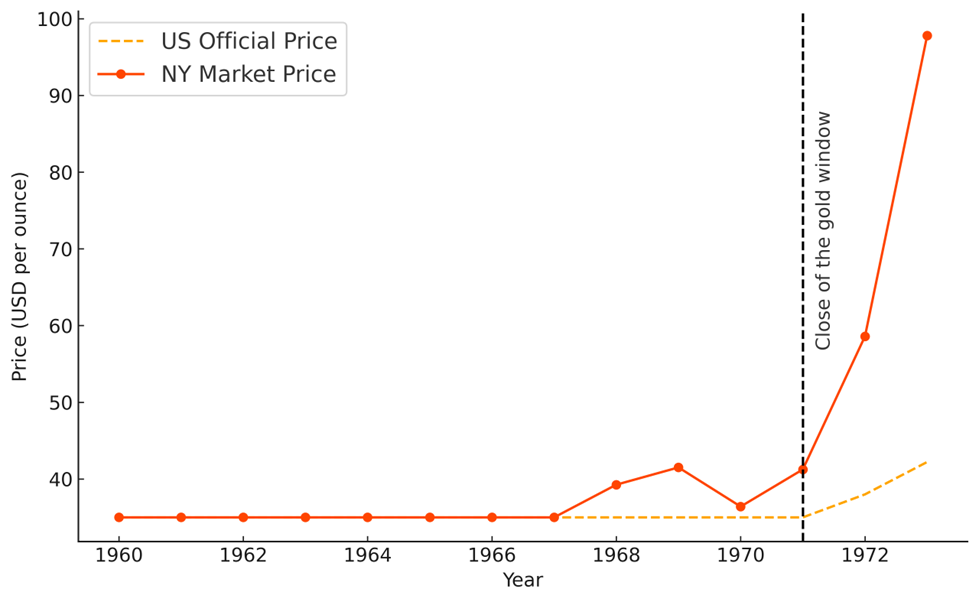
\includegraphics[width=0.9\linewidth]{figure2.png}
    \caption*{\small Source: Author's own elaboration based on \citet{officerwilliamson2025}. “The Price of Gold, 1257–Present.”
MeasuringWorth  .}
   \label{fig:gold_price}
\end{figure}

Figure~2 plots official and New York market gold prices from 1960 to 1973 and shows the widening gap between the official price at 35 dollars per ounce and market quotations, especially after 1968 and into 1972--73. The divergence signaled more than speculative turbulence. By dissolving the legal constraint of convertibility, the breakdown of Bretton Woods created space for financial capital to reassert command over the hegemonic bloc in power, taking control of monetary and macroeconomic policy in the U.S.\ and, by fiat standard, over the world market \citep{vernengo2021,alami2023}. Neoliberal economists had long supplied the ideological grammar for such a shift; \citet{friedman1953} framed fixed-rate coordination as a ``straitjacket'' on market adjustment. Abandoning convertibility thus functioned as a domestic hinge: it loosened capital controls that had kept funds within national borders and cleared the ground for redefinition of mainstream macro policy. The emergent consensus prioritized price stability and ``discipline,'' and it dismantled full-employment commitments and their social base. It also allowed the dollar to operate as a global reserve without the discipline of gold, reinforcing U.S.\ hegemony through financialization.

The collapse of American Keynesianism was not merely conjunctural; it was rooted in its intellectual architecture. Samuelson's \emph{Foundations} \citep{samuelson1947} and successive editions of \emph{Economics} \citep{samuelson1948} institutionalized the neoclassical synthesis, tying legitimacy to the performance of discretionary demand management. When stagflation exposed its weak flanks, the same apparatus that had legitimized Keynesianism became its gravedigger. Its technocratic ethos persisted through reconfiguration rather than abandonment: \citet{mahoneythelen2009} define this pattern as institutional conversion, a mode of gradual change where the rules remain formally intact but are strategically redeployed and enacted in new ways to serve new functions or purposes. The shift to credibility and rules could be narrated as theoretical refinement within the same disciplinary canon \citep{johnson2024}. Rational expectations and rules-based credibility displaced demand management while preserving continuity with neoclassical theory. In this reframing, capacity was re-coded as an inflation sentinel; profitability crises and the defeat of an emerging full-employment coalition reinforced a new form of state power: a move from Keynesian government towards neoliberal governance \citep{jessop2002}. The academic mainstream presented this as progress, thereby depoliticizing what was essentially a political defeat of organized labor and communities becoming a redistributive and anti-imperialist coalition. In other words, it was the awakening of the national community against the logic of capital (Garc{\'\i}a-Linera, [1994] 2000; \citealp{basu2022}) but ultimately defeated by the redistribution of power within capital itself.

Taken together, these dynamics show how capitalist-class agency, conjunctural constraints, and regime contradictions converged to re-anchor macroeconomic authority within a racialized political economy that had long circumscribed U.S.\ liberal democracy \citep{quijano2000,schiller2015}. In the emergent configuration, credibility and supply-side reform displaced demand management, while policymakers and economic advisors recoded capacity utilization from a Keynesian slack index into a mechanism for labor discipline, operationalized through the rhetoric of an inflation sentinel \citep{shaikhetal1999,johnson2024}. What followed was not simply the decline of a policy paradigm but a restructuring that reinscribed old hierarchies under new technocratic forms of de-democratizing American society \citep{gordonedwardsreich1982,kiely2016}. State officials and financial capital interests dismantled the Keynesian State, inaugurating neoliberal governance as an uneven, historically contingent process with multiple modalities and pathways unfolding within and beyond U.S. borders \citep{jessop2002,brenner2002,brennerpecktheodore2010}. The fall of American Keynesianism, in this sense, was a translation rather than an end: domestic racial fracture and international monetary restructuring transformed the U.S.\ dollar from world money under the Bretton Woods gold standard into fiat money at the core of a neoliberal order that carried forward long-standing hierarchies across the globe towards the era of neoliberalism \citep{harvey2007}.


\section{Conclusions}

This article has reconstructed the institutional history of capacity utilization measurement in three phases. First, it uncovered pre-Keynesian endeavors at the Brookings Institution to operationalize productive capacity as a policy-relevant statistic. Second, it documented how postwar debates consolidated survey-based benchmarks within the Federal Reserve's statistical apparatus, marginalizing engineering-based alternatives. Third, it analyzed the crisis of Fordism as a critical juncture in which emerging neoliberal figures reinterpreted high operating rates as inflationary warnings, thereby recoding capacity utilization from a slack indicator into a disciplinary device. This recoding was not a clean theoretical break but an instance of institutional conversion: the same technocratic toolkit that had legitimized American Keynesianism was redeployed to justify rules-based neoliberal governance.

This article contributes to multiple fields of inquiry. First, by shining a light on the contested and ideologically embedded nature of macroeconomic indices and how their interpretation expresses the discursive practices and operational routines of economic reasoning, it provides a new epistemological and historically situated angle to critically assess the revival of the so-called ``utilization controversy'' in heterodox macroeconomics. Originally developed in \emph{Political Economy: Studies in the Surplus Approach}, this controversy was triggered in response to \citet{amadeo1986}'s proposal about the endogeneity of the capacity utilization rate at normal operating conditions, i.e.\ its self-adjustment to demand conditions, as a means to resolve the unstable results of the Neo-Kaleckian growth model. In response, researchers under the umbrella of \citet{sraffa1960}'s reconstruction of Classical Political Economy responded to Amadeo's proposal vouching for an exogenous determination of the normal rate of capacity utilization \citep{kurz1986}. In a more nuanced response, \citet{ciccone1986} vouched for a weakly exogenous determination explained by the slow speed of adjustment to normal rates of operation due to firms' demand-management behavior, costs of adjustment, or the sluggish maturity of new productive capacities. Contemporarily, the controversy has been revisited by Nikiforos, aiming to provide empirical evidence on a previous contribution where an endogenous determination of capacity utilization in normal conditions is justified using micro-foundations \citep{nikiforos2013}. Reconstructing the time-series of capital's AWW, \citet{nikiforos2016} operationalized the debate econometrically, arguing that FRB capacity utilization measures are conditionally stationary by construction at given windows, while showing evidence favorable for an endogenous determination of normal capacity utilization once tested using physical measures. This intervention sparked a debate by a subsequent rebuttal in a critical econometrical replication by \citet{gahnGonzalez2020} followed by \citet{nikiforos2020}'s rejoinder, continued by parallel paths without further discussion among the authors.

By reconstructing the history of capacity utilization survey measures, this article suggests that many of the critiques of the institutionalization of macroeconomic indices and their subsequent methodological splices and adjustments should not be taken at face value, as extensively argued by critical inquiries such as the ones made by Shaikh in several interventions \citep{shaikh1992,shaikhmoudud2004,shaikh2016}. In this regard, the interpretation of the contribution to the long-standing debate in heterodox economics on the determination of a normal rate of capacity utilization is presented here suggesting that recovering plural measurement practices can inform contemporary debates over democratic macroeconomic governance, rather than taking a particular trench in the so-called ``utilization controversy.''

Second, the article highlights the role of macroeconomic indices in the broader political economy of distributive conflict and how the debate on capacity utilization measurement played a key role in a critical juncture of historical capitalism at the core of the world system. This provides a contribution to the emergent field of historical political economy, which in turn is understood as the intersection of political science, economics, and history \citep{jenkinsrubin2024hpe}. By digging into the history of Fordism in the United States and its crisis, the article shows clearly how prominent figures of mainstream macroeconomics throughout the post-Fordist era---marked by the dominance of neoliberal political thinking and the de-democratization of liberal society---were already incubated in the neoclassical synthesis expressed by the seminal works of Samuelson's \emph{Foundations} \citep{samuelson1947}, a highly influential account for graduate students and mainstream scholarship in the economics discipline, but more importantly highly influential in the cultural landscape of higher education as expressed in Samuelson's \emph{Economics} \citep{samuelson1948} and its multiple re-editions. As clearly defined by \citet{jenkinsrubin2024hpe}, the field of historical political economy aims to assess how research on dynamics and events from the past informs us about the present conditions we are living in. In this sense, the overview of the works and relevance in policymaking expressed in the figure of Alvin Hansen provides important insights on the role of intellectuals in society, which mirrors our present, also featured by secular stagnation in the United States and beyond \citep{cruztavani2023}.

Finally, the article contributes to the growing call among early-career scholars in International Political Economy and Development Studies to ``decolonize economics'' \citep{kvangravenkesar2023,duttalveskesar2025}. Unmasking macroeconomic indicators as ideological weapons shows how the re-coding of capacity utilization from a Keynesian slack index into an inflation sentinel served to police distributional conflict and narrow the space for democratic claims. This reveals, rather than obscures, the racialized core of U.S.\ liberal democracy and strengthens arguments about the de-democratization of American society \citep{kiely2016}. Crucially, the analysis refuses to treat Fordism as a closed national model and instead situates it within a global historical configuration of power: Atlantic Fordism as a multi-scalar bloc, Bretton Woods as a geopolitical architecture, and the dollar's post-1971 role as an instrument of worldwide financial discipline. In methodological terms, the paper draws on dependency theory as an open research program rather than a finished doctrine \citep{kvangraven2021}, using it to provincialize U.S.\ macroeconomic narratives and to foreground how external constraints, empire, and world-market hierarchies contour ``domestic'' policy space. This perspective also recovers subaltern political economies typically erased by mainstream macroeconomics. It registers how full-employment coalitions, civil-rights insurgencies, and community-based projects articulated alternative imaginaries of economic democracy that ran against profitability imperatives, and how technocratic redefinitions of ``capacity,'' ``credibility,'' and ``discipline'' neutralized those claims by translating them into putatively neutral metrics. In doing so, the article reframes indicators as historically situated infrastructures of governance and knowledge, rather than universal measures of truth.

In summary, the paper reframes capacity utilization not as a neutral thermometer but as a thermostat built into the machinery of state power: a device whose settings were engineered, contested, and ultimately recalibrated to discipline labor, narrow democratic horizons, and reorganize hierarchies of the capitalist world market. Tracing that recoding from Brookings surveys to McGraw--Hill benchmarks, Federal Reserve adoption, and the critical juncture of stagflation turned into rule-making shows how statistical infrastructures translated political choices into technical ``facts.'' Read this way, the fall of American Keynesianism was not a tidy paradigm shift but a struggle over who gets to define and conduct macroeconomic policy across a racialized and imperial order. Recognizing this history underscores the need to recover suppressed indicators and overlooked measurement practices, to build plural and transparent series tied to material production and social reproduction, and to reopen the policy dashboard to democratic contestation. If macro policy is government by numbers, then the numbers must be returned to politics, a necessary step for contemporary societies to face major challenges: de-link from stagnation trajectories, redistribute power, and design institutions capable of sustaining full employment and social rights.

% ---------- Bibliography ----------
\pagebreak
\bibliographystyle{apalike} % or your preferred style
\bibliography{references}

% If biblatex:
% \printbibliography

\end{document}
